\section{Experiment 10H-F: output identifiability and physical-score audit}
\label{sec:experiment10hf}

\paragraph{Question and parameterization.}
Experiment 10H-E found that generic innovation summaries do not reliably
separate the vehicle classes. Experiment 10H-F asks two more fundamental
questions: are physically meaningful LPV coefficients identifiable from the
complete measured-output prediction error, and do likelihood scores at a
common nominal model provide a better label-free grouping signal?

The estimator does not receive mass, inertia, tire stiffness, geometry,
relaxation lengths, actuator constants, latent states, client matrices, or
class labels. Instead, it operates in nine effective continuous-time LPV
coordinates:
\begin{equation}
 \theta=[a_f^r,a_r^r,q_f^\beta,q_f^r,q_r^\beta,q_r^r,
          s_f,s_r,s_\delta]^\top,
\end{equation}
where the first two coefficients map normalized axle forces to yaw
acceleration, the next four govern front/rear force response to sideslip and
yaw rate, $s_f$ and $s_r$ are relaxation decay rates, and $s_\delta$ is the
actuator rate. These combinations generate the structured $A(v;\theta)$ and
$B(v;\theta)$ matrices directly. They avoid claiming separate identification
of quantities such as $C_f$ and $m$ when only their combinations affect the
model.

\paragraph{Measured-output information.}
Each calibration segment begins with 100 zero-command samples to estimate the
trajectory-constant sensor offset, followed by the client's frozen 10H
frequency-band excitation. A KF at one fixed nominal design produces whitened
innovations. Central finite differences with a 0.02 log-parameter step give
the innovation Jacobian $J_i$. The local observed-information approximation
and physical score are
\begin{equation}
 F_i=J_i^\top J_i,
 \qquad s_i=J_i^\top\bar\nu_i.
\end{equation}
All quantities come from $r$, $a_y$, applied steering, steering command, and
speed. True classes are opened only afterward to aggregate compatible-client
information and evaluate clustering.

Across 300 development clients, 296 local information matrices have numerical
rank nine and four have rank eight at a relative $10^{-6}$ tolerance. Thus the
expected strict local-rank-deficiency mechanism does not occur. Local
identification is nevertheless weakly conditioned: the median condition
number is $5.95\times10^4$ and the maximum is $9.64\times10^5$. Every
compatible-class aggregate is full rank, with condition numbers between
$1.16\times10^4$ and $2.15\times10^4$. Sharing therefore improves numerical
conditioning and expected estimation variance rather than restoring literal
rank.

\paragraph{Physical-score grouping.}
Client scores are whitened by the fleet information matrix, residualized for
known speed-block effects, standardized, and clustered with the same
unknown-$K$ diagonal-GMM/BIC protocol as 10H-E. BIC selects one group in two
fleets, two groups in six fleets, and three groups in two fleets. Modal $K=2$
and the three-group rate is 20\%.

The retrospective fixed-$K=3$ diagnostic obtains mean ARI 0.209, mean balanced
accuracy 0.593, and minimum class recall zero. This is worse than the generic
10H-E innovation signature. A first-order score evaluated at one common
nominal point therefore does not represent the nonlinear distance between a
client trajectory and the eventual group models.

\begin{table}[htbp]
\centering
\caption{Experiment 10H-F development diagnostics.}
\label{tab:experiment10hf}
\begin{tabular}{lr}
\toprule
Diagnostic & Result\\
\midrule
Local full-rank fraction & 98.67\%\\
Median local information condition & $5.95\times10^4$\\
Maximum local information condition & $9.64\times10^5$\\
Compatible aggregates full rank & 30/30\\
Maximum compatible condition & $2.15\times10^4$\\
Modal BIC group count & 2\\
Fixed-$K=3$ mean ARI & 0.209\\
Fixed-$K=3$ balanced accuracy & 0.593\\
\bottomrule
\end{tabular}
\end{table}

\begin{figure}[htbp]
\centering
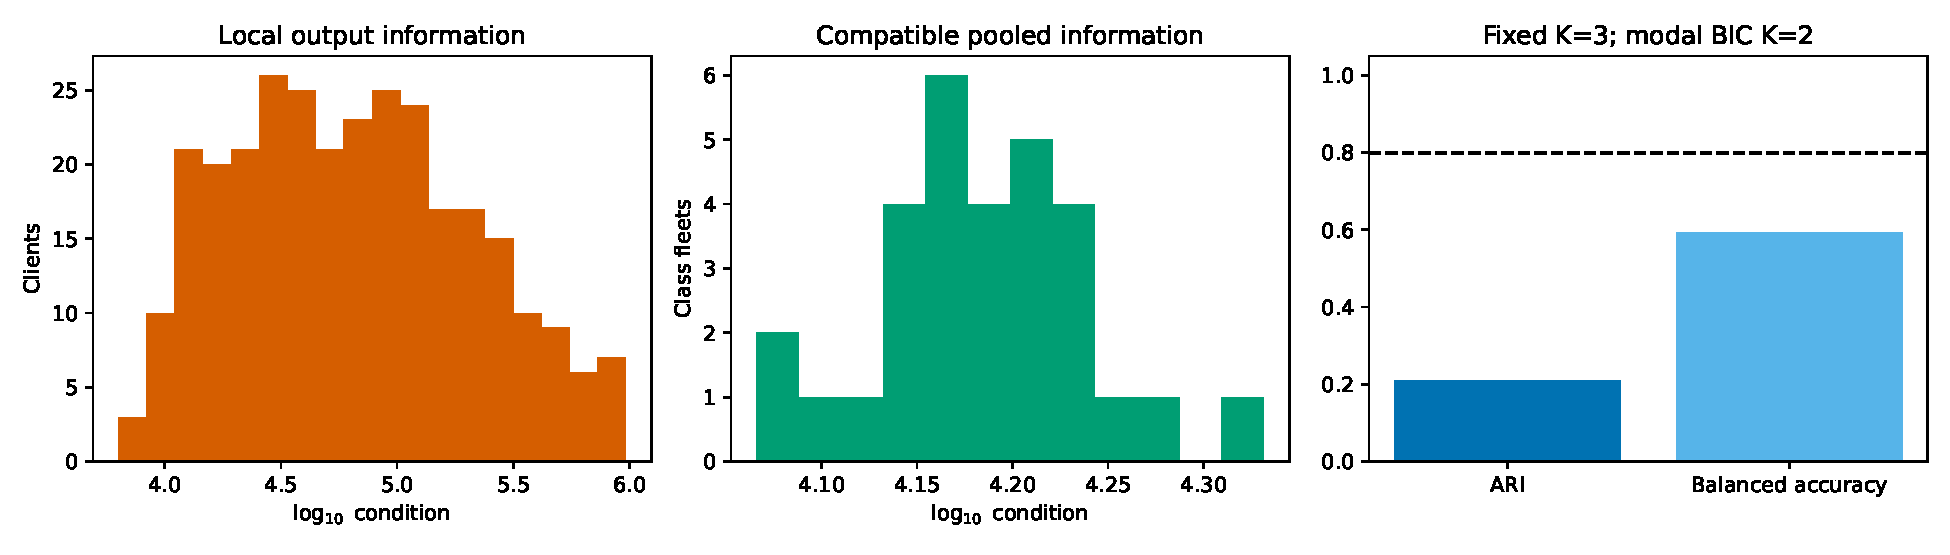
\includegraphics[width=0.98\linewidth]{../results/figures/experiment_10hf_output_identifiability.pdf}
\caption{Local and compatible-pooled information conditioning together with
fixed-$K$ physical-score clustering performance.}
\label{fig:experiment10hf}
\end{figure}

\paragraph{Gate decision and interpretation.}
The development gate fails. Its two parts have different implications. The
output-identifiability audit is encouraging: the selected effective
coordinates are visible, compatible aggregation is full rank, and pooling
improves conditioning. The clustering audit is negative: neither generic
innovation summaries nor a single nominal-point score reliably initializes
the physical groups.

Consequently, the next method should not hard-cluster first-order scores before
model learning. The defensible next gate is a structured global
prediction-error fit from measured outputs, with held-out likelihood and
parameter-profile diagnostics. If that optimizer reliably learns one physical
model without hidden-parameter initialization, it can be extended to a
known-$K$ multi-start mixture in which assignments and models evolve jointly.
Candidate mixture models should be generated by physically bounded
split-and-perturb restarts around the learned global model, not by true class
centers or client parameters. Confirmation seeds 591--600 remain sealed.

\paragraph{Reproducibility.}
Configuration and implementation are in
\path{code/config/experiment_10hf.json} and
\path{code/experiments/experiment_10hf_output_identifiability.py}.
Client information diagnostics, compatible and fleet aggregates, candidate
BIC scores, fixed-$K$ clustering metrics, gate decisions, leakage declaration,
reserved confirmation seeds, and provenance hashes are stored under
\path{results}.
